\documentclass{article}
%% PACKAGES %%

\usepackage{amsmath, amsfonts, amssymb, amsthm}
\usepackage{braket}
\usepackage{listings}
\usepackage{geometry}
\usepackage{xcolor}
\usepackage{textcomp}
\usepackage{graphicx}
\usepackage{fancyhdr}
\usepackage{sourcecodepro}
\usepackage{multirow}

%%%%%%%%%%%%%%

\graphicspath{{./images}}
\setlength\parindent{0pt}       % globally supress indentation

%% LISTINGS CONFIG %%

\definecolor{purple2}{RGB}{153,0,153} % there's actually no standard purple
\definecolor{green2}{RGB}{0,153,0} % a darker green

\lstset{
  language=Verilog,                   % the language
  basicstyle=\normalsize\ttfamily,   % size of the fonts for the code
  frame = single,
  % Color settings to match IDLE style
  keywordstyle=\color{orange},       % core keywords
  keywordstyle={[2]\color{purple2}}, % built-ins
  stringstyle=\color{green2},%
  showstringspaces=false,
  commentstyle=\color{red},%
  upquote=true,                      % requires textcomp
  numbers=left,
  breaklines=true,
}

% Title Stuff
\title{\vspace{-3cm} ECE426 Homework 8 \\ \textit{\normalsize Pipelined 12-bit Subtractor}}
\author{Chase A. Lotito, \textit{SIUC Undergraduate}}
\date{}

\begin{document}

\pagestyle{fancy}

% attempt to make nice header
\fancyhead{}
\fancyhead[CH]{\normalsize{LOTITO - SIUC ECE - SPRING 2024 - ECE426 HW8}}

\maketitle % Makes the title

\section*{Question}

Write Verilog code for subtracting two 12-bit numbers in 2's complement. Subtract 6 bits at a time to pipeline your design.

\bigskip

The \textit{subtractor.v} code below:

\begin{lstlisting}
/*
    Chase Lotito - SIUC
    ECE426 - HW8 - Pipelined Subtractor
*/

module subtractor (clk, n1, n2, subtract);

// I/O
input clk;
input [11:0] n1;
input [11:0] n2;
output [12:0] subtract;

reg [12:0] subtract;
wire [12:0] signe_n1;
wire [12:0] signe_n2;

reg [12:0] twosc_n2;
reg [12:0] n1_reg1;

wire [6:0] sub_lsb;
reg [6:0] sub_lsb_2;
reg [12:6] twosc_n2_2;
reg [12:6] n1_reg2;

wire [12:6] sub_msb;
wire [12:0] sub_next;

assign signe_n1 = n1[11] ? {1'b1, n1} : {1'b0, n1}; // sign extend n1
assign signe_n2 = n2[11] ? {1'b1, n2} : {1'b0, n2}; // sign extend n2

always @ (posedge clk) // Pipeline 1, clk (1)
begin
twosc_n2 <= ~signe_n2 + 1'b1; // compute twos complement of signe_n2
n1_reg1 <= signe_n1; // preserve n1
end

assign sub_lsb = n1_reg1[5:0] + twosc_n2[5:0]; // Add least 6 significant bits, sub_lsb [6] is the carry.

always @ (posedge clk) //pipeline 1, clk (2), register LSB to continue addition of MSB.
begin
sub_lsb_2 <= sub_lsb; // preserve LSB sum, sum_lsb_2 [6] is the carry.
twosc_n2_2 <= twosc_n2[12:6]; // preserve MSB of n2 for further processing.
n1_reg2 <= n1_reg1[12:6]; // preserve MSB of n1_reg1
end

// Add msbs with carry.
assign sub_msb = n1_reg2 + twosc_n2_2 + sub_lsb_2[6]; // add MSBs with carry
assign sub_next = {sub_msb, sub_lsb_2[5:0]}; // put together MSB & LSB of the final result

always @ (posedge clk) // Pipeline 2, clk (2), register the final result
begin
subtract <= sub_next;
end

endmodule
\end{lstlisting}

The testbench:

\begin{lstlisting}
// chase lotito - subtractor testbench for HW8

`timescale 1us / 1us
`include "subtractor.v"

module tb();

// GTKWAVE (waveform simulator)
initial begin : GTKWAVE
    $dumpfile("tb.vcd");
    $dumpvars(0, tb);
end

// I/O
reg clk;
reg [11:0] n1, n2;
wire [12:0] subtract;

// Initialize subtractor
subtractor U1
(
    .clk(clk),
    .n1(n1),
    .n2(n2),
    .subtract(subtract)
);

initial begin : start
    clk = 1'b0;
end

// CLOCK
always begin : clock
   #10 clk = ~clk;
end

// stimulus for subtract = n1 - n2
initial begin : stimulus
    n1 <= 0;
    n2 <= 0;
    #10;
    n1 <= 10;
    n2 <= 5;
    #30;
    n1 <= 60;
    n2 <= 50;
    #100 $finish;
end

endmodule
\end{lstlisting}

This gives the following waveforms. As we can see the 3 following subtractions were computed: \(0-0=0\), \(10-5=5\), and \(60-50=10\).

\begin{figure}[!ht] 
    \centering
    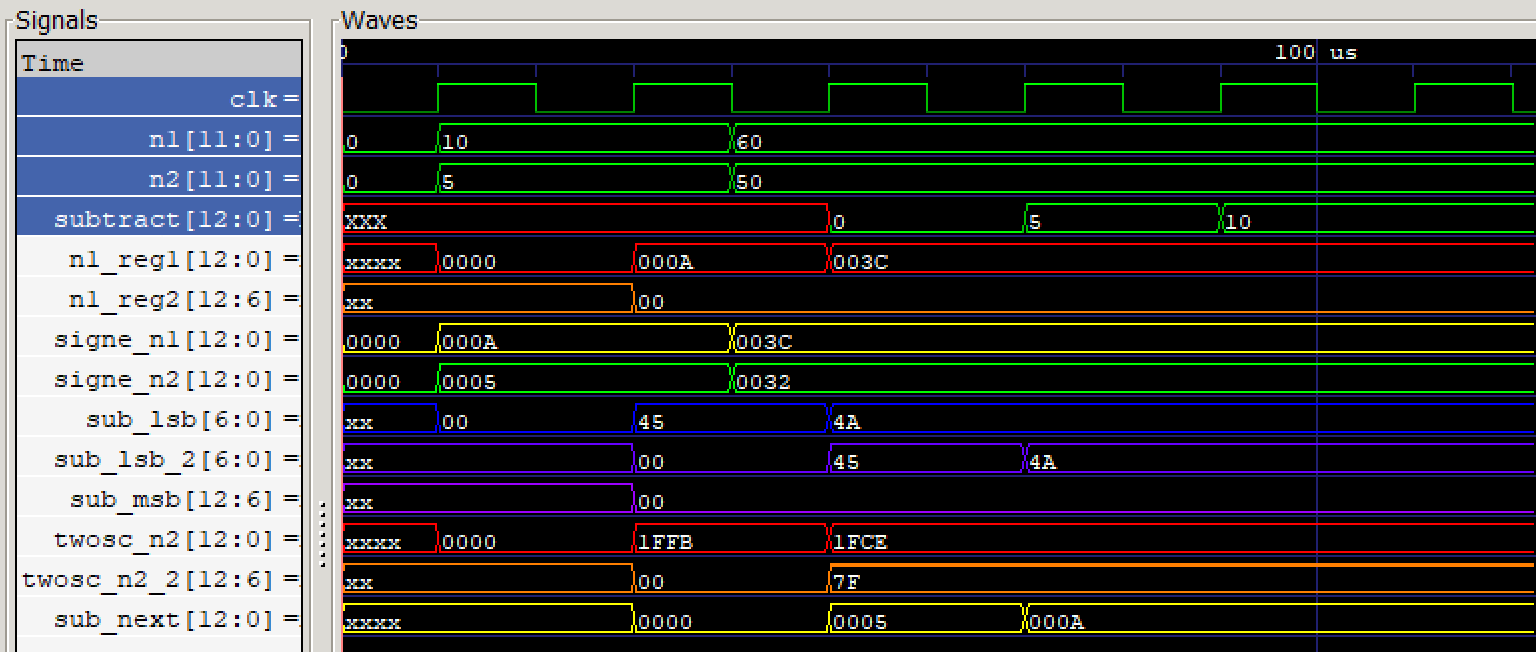
\includegraphics[width = 15cm]{waves.png}
    \caption{Waveforms for pipelined 12-bit Subtractor}
    \label{fig:waves}
\end{figure}

\end{document}
